\section{Software: Governing machine protocols and stimulus presentation}
\label{sec:sectionc}

Bpod's software allows to load user-made protocols and run them within the built-in bpod interface, joined with the protocols' specific GUI windows (IMAGE).

In this project, three protocols were developed for different ends: receptive field mapping, tuning measuring and studying the spatial structure of surround modulation.

Each of these were subsequently used in mice experiments. The produced data was also analysed, validating the method and tool in the three protocols. 

The RF protocol served to find the RF positions after each experimental session and assess if the majority of the measured cells' RFs was centred at the corresponding display monitor center, as desired. Specifically, the obtained RF maps either indicated, in combination with the retinotopy maps, in which directions one should move the objective to correct the imaging position in following sessions or confirmed that the objective and mouse placing was appropriate (SEE CHAPTER). Furthermore, this data was also combined with the SM protocol's results for RF position-dependent analysis of the SM effect (SEE CHAPTER).

The tuning protocol was implemented to measure the selectivity of cells in a flexible array of conditions. The data collected from this protocol was analysed and some cell's tuning behaviour examples are shown in (SEE CHAPTER). This analysis served to validate the protocol and aided in troubleshooting the SM analysis. Moreover, this protocol was also used to find the RF centred imaging positions during experiments. 

Finally, the SM study was the main focus of this project's experimental component, and the obtained results are presented in (SEE CHAPTER). The implementation of this protocol allows the presentation of any configuration with center and surround moving gratings' patches, in any combination of the four cardinal plus center positions. For this project's purposes, 124 were chosen, in a given set of grating frequencies and stimuli sizes (SEE CHAPTER).

Each of these protocols follows a similar structure of five files, each with different case functions:

\begin{itemize}
\item \textbf{main}: initiate, submit, start, prepare next trial, synchronize GUI, save settings and events, process trial completed, restart and stop;
\item \textbf{states matrix}: prepare matrix, run;
\item \textbf{GUI}: initialize, synchronize;
\item \textbf{SoftCode handler instructions}: maps SoftCode bits to be sent in the states matrix to functions: main(prepare next trial), main(save settings events) and main(synchronize GUI);
\item \textbf{Support functions}: set session, set next stimulus and save parameters.
\end{itemize}

In bpod's built-in interface, one can set the mouse ID, load the settings to use as default and then call the desired protocol. 

At this point, the main file is called to initiate the protocol: This by its turn calls the GUI initiation function, which initializes the settings variables in a global structure S, in different fields according to the required type of GUI to be used (an edit box, a toggle button, a slider, an edit array, an array display or a push button). This organization allows to then easily initialize handles of each parameter's user interface control, depending on the type of GUI (IMAGES).

Once the user chooses the intended parameter values in the GUI and clicks the \textit{submit} button, the GUI is synchronized, the current trial variable is set to 1 and three support functions are run on S: 

First, the session is set: An angular coordinate system is computed, converting monitor $(y,z)$ coordinates in azimuth and elevation, from the perspective of the mouse:

\begin{equation}
elevation(º)= - \left[ \dfrac{\pi}{2} - \arccos \left( \dfrac{z+z_0}{\sqrt{d^2 + (y + y_0)^2 + (z+z_0)^2}} \right) \right] \dfrac{180}{\pi}
\end{equation}

\begin{equation}
azimuth(º)= \dfrac{\arctan(y-y_0)}{d}\dfrac{180}{\pi}
\end{equation}

with $y_0$ and $z_0$ the positions in respectively the horizontal and vertical monitor axis centred perpendicularly to the mouse's gaze and $d$ the distance from the mouse eye to the center monitor position.

In the RF case, grid positions can be produced from the settings and randomly permuted in a presentation sequence, along with a key for the respective gratings direction sequence also in pseudo-randomized order.

The second support function sets the next stimulus, by updating the current stimulus variables to the first trial case, according to the order in the total stimuli arrays created at the beginning of the session (position and direction sequence for the RF protocol).

Then, in the third support function, the relevant parameters for the stimuli graphical presentation are saved in an external \textit{next stimulus} file, to be read and loaded in the psychtoolbox stimuli display Matlab instance.

The GUIs are synchronized to the newly computed values of the parameters, and the states matrix' preparation is called.

The matrix sent to the bpod device follows the flowchart in figure ??.

\begin{figure}[H]
	\centering
		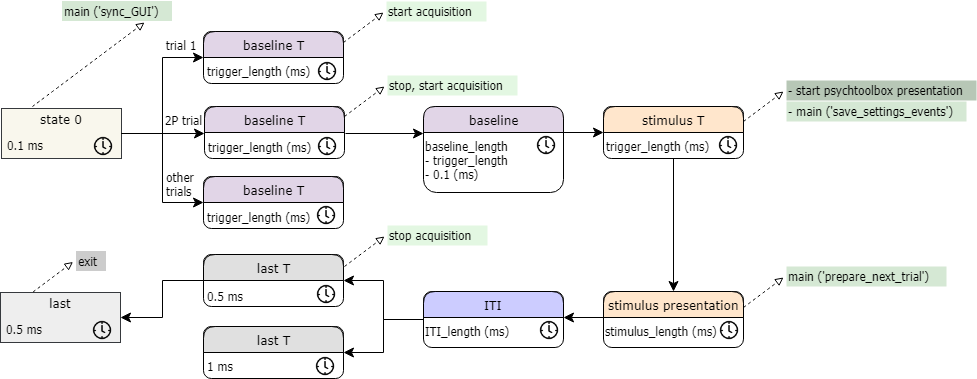
\includegraphics[width=1\linewidth]{3.Chapter/bpodimplementation.png}
	\caption[c1]{Flowchart of the states matrix implemented for the three developed protocols (RF, Tuning and SM). Each state is represented by a name, a timer, state change conditions and output actions. The states machine is formed by three principal states: a baseline, a stimulus display and an ITI. Trigger ("T") states were added, with \textit{trigger length} times corresponding to the duration of the according pulse. All of the state changes were to happen at the end of the internal timer at the current state. The output actions are represented by dashed arrow lines: these represent triggers to the imaging computer (lighter green) through BNC connections, to the NIDAQ of the psychtoolbox matlab instance (darker green) through a wire connection and internal triggers to other functions in the governing machine, through USB connected softcodes (meddium green).}
	\label{fig:bpodimplementation}
\end{figure}

After this \textit{submit} process, the user can initiate the psychtoolbox script written for the given protocol at use, in a second matlab instance. This script opens the NIDAQ device and configures it to receive triggers, then opens the screen in the setup monitor in front of the mouse, and loads the session settings in the \textit{next stimulus} file. For the case of the RF, this computes a checkerboard mask and divides it into a mask for each grid cell's position figure. It also prepares full screen gratings at the settings' frequencies and contrast levels, going in the indicated sequenced directions. Finally, these are combined into textures - sequences of images - that correspond to each trial type and that are saved in a structure for that trial type and every frame of that trial.
When a trigger reaches the entrance specified in the NIDAQ device, the corresponding trial texture frames are drawn in sequence and the timing between the previous trigger and the current one is displayed on the matlab command window for monitoring possible skipped triggers.

When the textures are loaded, the user can click the start button, which first saves the submitted settings in a stimulus file and then calls the states matrix to run.

As represented in IMAGE??, a \textit{prepare next trial} instruction is sent in the middle of each trial. In parallel to the stimulus presentation, this instruction increments the current trial variable, then runs the \textit{set next stimulus} support function and calls the \textit{prepare next matrix} function. This ensures that the next trial variables, GUI and matrix are ready when the current trial finishes and the next \textit{run states matrix} instruction is sent.

save settings events
sync GUI
trial completed
restart, stop. calibration, reset nidaq

SM, tuning, explain support functions and psychtoolbox

diagram of a mini session

\subsection{Implementation and hardware alterations}
\label{subsec:subbsectionC}

\subsection{Stimulus presentation with psychtoolbox}
\label{subsec:subdsectionC}

\subsection{Optical imaging with Scanimage interface}
\label{subsec:subesectionC}